%!TEX root = ../schoedon.tex

\cleardoublepage
\chapter{Overview and related work}
  \label{chap:overv}

  Foo.\par

  \section{Accessibility analytics and mapping techniques}
    \label{sec:overv:accss}

    Table \ref{tab:overv:relat} (page \pageref{tab:overv:relat}) shows a first
    overview of related graphics, applications and publications in the broad
    field of mobility analytics and accessibility mapping techniques.\par

    Back in 1881, Francis Galton created the Isochronic Passage Chart for the
    Royal Geographic Society (figure \ref{fig:overv:isopc}). It depicts the world
    as a thematic map with an overlay of colour-coded isochrones to show the
    distances that can be traveled in equal times. It uses the isochronic
    visualization as a rough generalization and suggests future areas of
    application might be \enquote{continental travel} or \enquote{home
    excursions} \cite{galton1881construction}.\par

    \begin{figure}[htb]
      \centering
      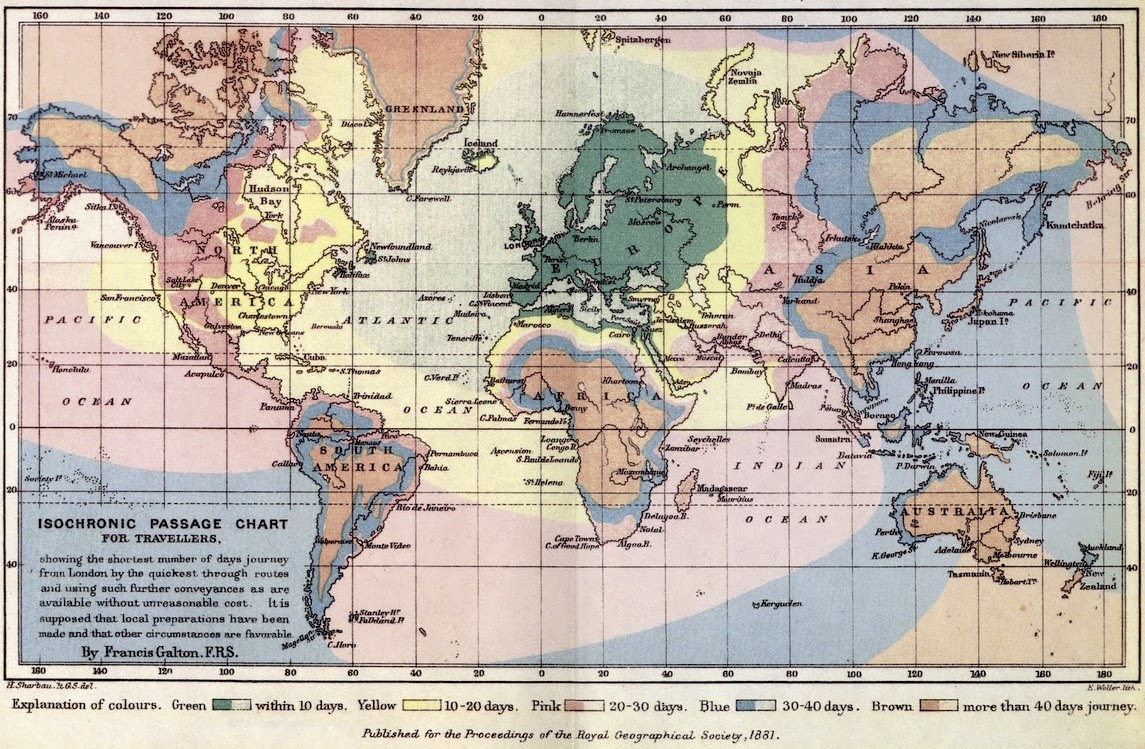
\includegraphics[width=\linewidth]
        {./img/overv-isopc.jpg}
      \caption{The Isochronic Passage Chart by Francis Galton, 1881 \cite{galton1881construction}.}
      \label{fig:overv:isopc}
    \end{figure}

    Google issued a patent in the United States of America on the
    \enquote{Method of Providing Travel Time} (compare figure
    \ref{fig:overv:patnt}).\par

    \begin{figure}[htb]
      \centering
      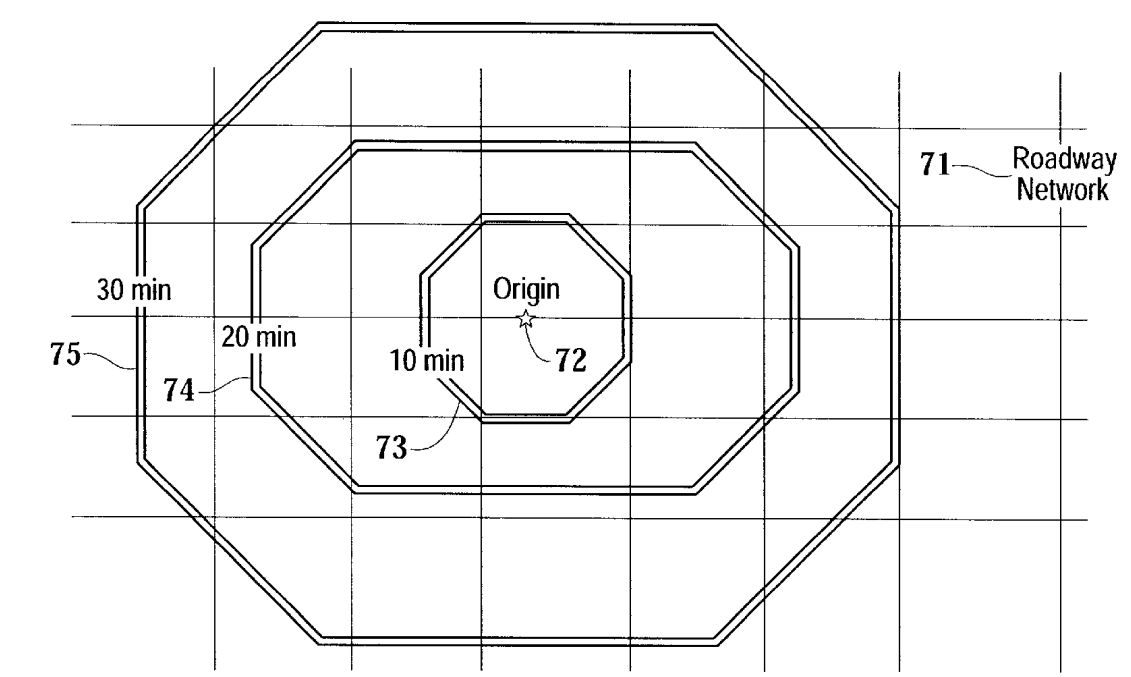
\includegraphics[width=\linewidth]
        {./img/overv-patnt.png}
      \caption{The Method of Providing Travel Time by Bin Ran, 2000 \cite{ran2001method}.}
      \label{fig:overv:patnt}
    \end{figure}

    % pubs %%%

    % galton first isochronic passage chart 1881

    %

    % ran google patent travel time 2001

    % street thesis application isocrones as transportation network costs display 2006

    % van campenhout summary overview travel time maps 2010

    % glander 2010

    % müller 2010

    % hollburg 2012

    % gortana 2014

    % hollburg 2014

    % maps %%%

    % apps %%%

    \begin{table}[htb]
      \tiny \centering
      \begin{tabular}{r|l|l|l|c}
       \textbf{Year} & \textbf{Authors} & \textbf{Contribution} & \textbf{Type} & \textbf{S} \\
       \hline
        1881 & Galton \cite{galton1881construction} & Construction of isochonic passage-charts  & Graphic  & * \\
        1972 & Armstrong \cite{armstrong1972network} & Network analysis of airport accessibility  & Publication  & \\
        1978 & Muller \cite{muller1978mapping} & Mapping of travel times  & Publication  & \\
        1981 & Sugiura \cite{Sugiura1981} & Japan travel time maps  & Graphic  & \\
        1986 & Hall \cite{hall1986fastest} & Network with random time-dependent travel times  &  Publication & \\
        1989 & Cauvin et al. \cite{cauvin1989cartographic} & The piezopleth maps method  & Publication  & \\
        1993 & Spierkermann et al. \cite{spiekermann1993zeitkarten} & Time maps for spatial planning  & Publication  & \\
        1994 & Spierkermann et al. \cite{spiekermann1994new} & Time-space maps of Europe  & Publication  & \\
        1996 & Gutierrez et al. \cite{gutierrez1996accessibility} & Accessibility analysis of the European road network  & Publication  & \\
        1998 & Fritz et al. \cite{fritz1998accessibility} &  Accessibility as wilderness indicator  & Publication  & \\
        1999 & Spiekermann \cite{spiekermann1999visualisierung} & Visualization of railway travel times & Publication & \\
        2000 & O'Sullivan et al. \cite{o2000using} & Using desktop GIS for accessibility analysis in public transport  & Publication  & \\
        2001 & Ran \cite{ran2001method} &  Method of providing travel time  & Patent & * \\
        2002 & Lovett et al. \cite{lovett2002car} & Accessibility of general practitioner services  & Publication  & \\
        2003 & Dailey et al. \cite{dailey2003design} &  Multi-modal transit management system & Publication  & \\
        2005 & Auxhausen \cite{axhausen2005zeitkarten} & Time-maps of Switzerland  & Publication  & \\
        2005 & Chronomap \cite{Chronomap} & Drive-time analysis  & Application  & \\
        2005 & Karlin \cite{Karlin2005}  & London subway travel times  & Graphic & \\
        2005 & McLaren \cite{McLaren2005} & Time travel with the London tube map  & Graphic  & \\
        2005 & Travel Time Tube Map \cite{Carden2006} & Interactive travel time tube map  & Application  & \\
        2006 & Lightfoot \cite{Lightfoot2006} & Use-cases for travel time maps  &  Publication  & \\
        2006 & Pfoser et al. \cite{pfoser2006dynamic} &  Dynamic travel time maps & Publication  & \\
        2006 & Rüegg \cite{Ruegg2006} & Impact of public transport on travel times  & Poster & \\
        2006 & Street \cite{street2006timecontours} & Isochrone visualization to describe transport network costs  & Master's Thesis  & * \\
        2007 & Irving \cite{Irving2007} & Use-cases for travel time maps  & Publication  & \\
        2007 & Nies et al. \cite{neis2007webbasierte} & Web-based accessibility analysis  & Publication  & \\
        2008 & Bauer et al. \cite{bauer2008computing} & Isochrones in multi-modal transportation networks  & Publication  & \\
        2008 & Mapumental \cite{Mapumental}  &  Maps that show time & Application  & \\
        2008 & Uchida et al. \cite{Uchida2008} & Travel time to major cities  & Graphic  & \\
        2009 & FreeMapTools \cite{Freemaptools} & How far can I travel  & Application  & \\
        2009 & Uchida et al. \cite{uchida2009agglomeration} & Measure of urban concentration  & Publication  & \\
        2010 & Antrim et al. \cite{antrim2013many} & Use-cases for GTFS data & Publication  & \\
        2010 & Campenhout \cite{van2010travel} & Travel time maps  & Master's Thesis  & * \\
        2010 & Glander et al. \cite{Glander2010} & Accessibility maps to visualize quality of mobility  &  Publication & * \\
        2010 & Lei et al. \cite{lei2010mapping} & Mapping transit-based access  & Publication  & \\
        2010 & Marciuska et al. \cite{marciuska2010determining} & determining objects within isochrones  & Publication  & \\
        2010 & Müller et al. \cite{Mueller2010} & Distance transformations for accessibility mapping  &  Publication & * \\
        2010 & Time Maps \cite{TimeMaps} & Public transport time maps of the Netherlands & Application  & \\
        2011 & Birchler \cite{birchler2011computing} & Isochrones in multi-modal public transport networks  & Bachelor's Thesis  & \\
        2011 & Gemmel \cite{gemmel2012hedonic} &  Effects of walkability and public transit & Master's Thesis  & \\
        2011 & Gamper et al. \cite{gamper2011defining} & Defining isochrones in multi-modal spatial Networks & Publication  & \\
        2011 & Isochrone.ch \cite{IsochroneCh}  & Isochrones in schedule-based public transport  & Application  & \\
        2011 & Li et al. \cite{li2011dynamic} & Dynamic accessibility mapping  & Publication  & \\
        2011 & Söderström \cite{soderstrom2011personal} & Internet-driven maps based on time distances  & Publication  & \\
        2012 & Byrd \cite{Byrd2012} & Visualizing urban accessibility  & Publication  & \\
        2012 & Gamper et al. \cite{gamper2012scalable} & Computation of isochrones with network expiration  & Publication  & \\
        2012 & Conveyal \cite{Conveyal} & Transportation - land use analysis  & Application  & \\
        2012 & Hollburg et al. \cite{hollburghier} & Interactive accessibility analysis in Potsdam & Publication  & * \\
        2012 & Mapnificent \cite{Mapnificent}  & Web-based reachability visualization of public transport  & Application  & \\
        2012 & Mertens \cite{meertens2012} & Travel Time Maps of urban areas in the Netherlands  & Graphic  & \\
        2012 & TripTropNYC \cite{TriptropNYC} & Web-based accessibility visualization in New York  & Application  & \\
        2013 & Innerebner \cite{Innerebner2013} & Isochrones in multi-modal spatial networks  & PhD Thesis  & \\
        2013 & Innerebner et al. \cite{innerebner2013isoga} & Web-based geospatial reachability analysis tool  & Publication  & \\
        2013 & Transit Time NYC \cite{TransitTimeNYC} & Web-based subway transit times in New York & Application & \\
        2013 & Tran et al. \cite{tran2013go_sync} & Synchronizing transit data between GTFS and OSM  & Publication  & \\
        2014 & Gortana et al. \cite{gortanaisoscope} & Visualizing temporal mobility variance  & Publication  & * \\
        2014 & Hollburg \cite{Hollburg2014} & Interactive analysis and visualization of accessibility & Master's Thesis  & * \\
        2014 & Isoscope \cite{Isoscope} & Visualizing mobility with isochrone maps  & Application  & \\
        2014 & Route360° \cite{Route360} & Web-based travel time analysis  & Application  & \\
        2014 & Krismer et al. \cite{krismer2014incremental} & Incremental calculation of isochrones  & Publication  & \\
        2014 & Voll \cite{vollerreichbarkeiten} & Accessibility analysis of the Alps  & Publication  & \\
        2015 & TravelTimePlatform \cite{TravelTimePlatform} & Search and filter by time not distance  & Application  & \\
        2015 & Yin et al. \cite{yin2015understanding} & Web-based accessibility analysis and travel time displays  & Publication  & \\
        2016 & Schoedon et al. \cite{STHD2016} & Web-based visualization of transportation networks  & Publication  & * \\
      \end{tabular}
      \caption{135 years of related work.}
      \label{tab:overv:relat}
    \end{table}

  \section{Geographic visualizations of transportation networks}
    \label{sec:overv:geovs}

  \section{Web-based mapping components and services}
    \label{sec:overv:webmp}

  \section{Web-based rendering technologies}
    \label{sec:overv:webrn}



%%%%%%%%\chapter{Overview and related work}
%%%%%%%%  \label{chap:overv}

  %  Related work comprises basically accessibility map visualization, web-based
  %  visualization frameworks, and the rendering of transportation networks using
  %  GPUs. Glander et al. present an accessibility map visualization technique
  %  with a focus on polygon-based approaches~\cite{Glander2010}, and raster-based
  %  distance transforms~\cite{Mueller2010} which both lack precision in display
  %  offered by our approach. In~\cite{Yin2015}, a web-based system for visualization
  %  of multi-modal accessibility for multiple
  %  land-uses is presented. However, the visualization technique does not focus on the
  %  specifics of transportation network representations. Altmaier et al. (2003) was
  %  among the first to outline issues in web-based geovisualization
  %  applications~\cite{Altmaier2003}. In~\cite{Brabec2007}, challenges, requirements,
  %  and concepts of client-based browsing of spatial data on the World Wide Web are
  %  discussed. The presented system is based on a Java-Applet and does not exploit
  %  modern web technologies for rendering complex spatial data. Vaaraniemi et al. (2011)
  %  as well as Trapp et al. (2015) develop and evaluate approaches for transport network
  %  visualization utilizing modern graphics hardware \cite{Vaaraniemi2011,Trapp2015}.
  %  However, the presented rendering techniques can currently not be implemented
  %  using technologies for browser-based rendering and do no cover specifics of
  %  data representation and formats.\par

  % one way of communicating mobility information such as travel times are two dimensional maps
  % accessibility and mobility becomes a central topic in a growing number of fields
  % there are strong demands for corresponding web mapping components
  % based on massive geodata sets, such as osm

%%%%%%%%  \section{Accessibility analytics and mapping techniques}
%%%%%%%%    \label{sec:overv:accss}

%    A general motivation on web-based accessibility map applications in the context of geospatial analytics offers Hollburg et al. (2012) \cite{hollburghier}.\par

%    Glander et al. (2010) researches on visualization of accessibility maps with focus on polygon-based approaches \cite{Glander2010}.\par

    % isochronic passage chart (1881)
    % shortest path problem classes
    % Single pair shortest path (A to B)
    % Single source shortest path (A to N)
    % All pairs shortest path (N to M)

%%%%%%%%  \section{Geographic visualizations of transportation networks}
%%%%%%%%    \label{sec:overv:geovs}

    %Vaaraniemi et al. (2011) as well as Trapp et al. (2015) develop and evaluate solutions for transport network visualization utilizing modern computer graphics \cite{Vaaraniemi2011}\cite{Trapp2015}.\par

%%%%%%%%  \section{Web-based mapping components and services}
%%%%%%%%    \label{sec:overv:webmp}

    %Altmaier et al. (2003) was among the first to outline issues in web-based geovisualization applications \cite{Altmaier2003}. Klimke et al. (2011) proposed a camera path specification for geovisualization services on the web and mobile devices \cite{klimke2013service}.\par

%%%%%%%%  \section{Web-based rendering technologies}
%%%%%%%%    \label{sec:overv:webrn}

    %Both Coughlin (2013) and Trevett (2013) deliver outstanding motivations on why we need a standardized data format close to hardware devices for 3D applications on the web \cite{Coughlin2014}\cite{Trevett2012}.\par

    % raster, java, webgl
